\newpage
\part{Recursividad}
\setcounter{section}{0}

En Ciencias de la Computación, la programación imperativa es un paradigma de programación que describe a un programa en términos del estado de dicho programa y las instrucciones que cambian este estado. Entre dicho conjunto de instrucciones se encuentran los procedimientos/funciones (i.e. unidades invocables), los cuales definen una secuencia de operaciones que realizan una tarea específica y que pueden ser invocados desde cualquier sección de un programa.

En una unidad invocable $U_1$ el conjunto de instrucciones que se ejecutan siguen un secuenciamiento: $inst_1$, $inst_2$, ..., $inst_k$. Ahora, si alguna de las instrucciones corresponde a una llamada a otra unidad invocable $U_2$ entonces se crea un nuevo ambiente de programa y se ejecutan las instrucciones de ésta.

\begin{center}
	\textit{¿Qué sucede si una instrucción dentro de $U_1$ invoca a la unidad $U_1$?}
\end{center}

Para entender mejor este aspecto, vamos a estudiar la Recursión.


%%%%%%%%%%%%%%%%%%%%%%%%%%%%%%%%%%%%%%%%%%%%%%%%%%%%%%%%
\section{Definiciones} \label{lb:recursi}

La recursión es un proceso de definir una propiedad, una operación o una función en términos de sí misma. Así, es posible definir un conjunto ``infinito" de objetos/operaciones con una declaración finita. En términos de Algoritmia, un algoritmo recursivo contiene en sus instrucciones una invocación a sí mismo. El número de invocaciones recursivas debe garantizar la finalización de un bloque de instrucciones.

Un ejemplo de conjunto definido de forma recursiva son los números naturales, donde:
\begin{enumerate}
\item $0$ es un número natural que pertenece a $N$
\item $n$ pertenece a $N$, entonces $n+1$ pertenece a $N$
\end{enumerate}

La recursión también se puede observar en la naturaleza como la forma de un copo de nieve, o la hoja de helecho. Igualmente, cuando se coloca un espejo frente a otro sucede que el reflejo de un espejo se observa en el otro que contiene el reflejo del primero y así de forma sucesiva hasta que se hace imperceptible dicho reflejo.

Existe una técnica de programación conocida como divide y conquista (\textit{divide and conquer}) que consiste en dividir un problema en dos o más sub-problemas del mismo tipo (o muy similar) y del mismo tipo, hasta que su solución sea simple. La recursión es una herramienta vital en la técnica de \textit{divide and conquer}, donde una invocación recursiva resuelve un problema de menor tamaño, de forma sucesiva, hasta llegar a un problema que su solución sea directa o muy simple. Posteriormente, cada solución obtenida se debe combinar para obtener la solución final al problema original.

Por ejemplo, la función Factorial de un número $n$ se puede expresar como:

$$
n! = \left\lbrace
\begin{array}{ll}
\textup{si } n=0 & \Rightarrow 1\\
\textup{si } n\geq 1 & \Rightarrow n \times (n-1)!
\end{array}
\right.
$$

Si la operación $n!$ se define como una función llamada Fact con parámetro $n$, se puede definir la función factorial como:

\begin{lstlisting}[upquote=true, language=pseudo]
Fact(0) = 1
Fact(n) = n*Fact(n-1) //n > 1
\end{lstlisting}

Del mismo modo, la sucesión de Fibonacci se puede expresar algorítmicamente como invocaciones a una función Fib con parámetro $n$, expresada como:

\begin{lstlisting}[upquote=true, language=pseudo]
Fib(0) = 0
Fib(1) = 1
Fib(n) = Fib(n-1) + Fib(n-2) //n > 1
\end{lstlisting}

A continuación, estudiaremos que elementos componen a un algoritmo recursivo para su construcción.

%%%%%%%%%%%%%%%%%%%%%%%%%%%%%%%%%%%%%%%%%%%%%%%%%%%%%%%%
\section{Algoritmo Recursivo}

En un algoritmo recursivo se deben identificar 3 elementos primordiales:
\begin{enumerate}
\item Caso(s) base(s): Corresponde con los casos del problema que se resuelven con un segmento de código que no aplica recursividad. Normalmente, corresponden a instancias del problema simples y fáciles de implementar cuya solución es conocida. Ejemplo: Fact(0) = 1.
\item Caso(s) recursivo(s): Se refiere a los casos que se resuelven mediante invocaciones a sí mismo, y por lo general reduce el problema de dimensión para que se aproxime cada vez más a un caso base y pueda ser resuelto de forma simple. El caso recursivo contiene una operación vital que se refiere a la combinación de las soluciones parciales encontradas. Generalmente, esta operación constituye una función de mezcla, operación aritmética, etc.
\item Parámetros: En toda unidad invocable recursiva se requiere al menos un parámetro que debe ser modificado en cada invocación recursiva (reduciendo el tamaño del problema). Los parámetros de la unidad invocable recursiva serán utilizados (generalmente por valor) en cada instancia para resolver el problema.
\end{enumerate}

Para identificar los elementos mencionados, estudiemos la función Fact que calcula el factorial de un número.

\begin{lstlisting}[upquote=true, numbers=left, language=pseudo]
function Fact (Integer iN) : Integer
  if iN <= 0 then
    return 1
  else
    return iN * Fact(iN - 1)
  end
end
\end{lstlisting}

El caso base viene dado cuando el número a calcular es igual a $0$ (línea 2), donde la función retorna el valor de $1$ (línea 3). El caso recursivo se deriva directamente de la fórmula de la función factorial $n! = n*(n-1)!$, devolviendo el valor de $iN * Fact(iN -1)$ (línea 5). El parámetro empleado solamente es el número a calcular (línea 1), el cual va disminuyendo de uno en uno en cada nueva invocación.

En la mayoría de lenguajes de programación y en arquitecturas basadas en una pila (\textit{stack}), cuando se invoca a una función de este tipo, se crean instancias de la función donde se aloje la información necesaria en cada invocación para la ejecución de la función. Entonces, ¿qué efectos produce una invocación recursiva a nivel de ejecución en un computador?.

%%%%%%%%%%%%%%%%%%%%%%%%%%%%%%%%%%%%%%%%%%%%%%%%%%%%%%%%
\section{Ejecución}

Cuando se invoca a un procedimiento o función, se almacena el ambiente local de éste en el tope de la pila del programa donde se aloja. Dicho ambiente contienen los parámetros y demás variables locales. La unidad invocable podrá acceder a sus variables según las reglas de alcances definidas por el lenguaje de programación. Si una unidad invocable recursiva contiene variables locales y/o parámetros, se creará un nivel en la pila diferente por cada invocación. Los identificadores de las variables locales serán los mismos, pero en cada nivel recursivo son un grupo nuevo de variables, con posiciones de memoria distintas (i.e. distintos ambientes de referenciación).

Del mismo modo como se apilan las variables, se guarda la posición de la última instrucción ejecutada, de manera tal que, cuando la función termina, todo el ambiente local se desapila y se retorna el control al punto en donde se hizo la invocación. Los resultados pueden ser retornados, o dejados en variables pasadas por referencia, en atributos, o en variables globales.

%%%%%%%%%%%%%%%%%%%%%%%%%%%%%%%%%%%%%%%%%%%%%%%%%%%%%%%%
\section{Clasificación}

Existen diversos aspectos para la clasificación de unidades invocables recursivas $U_i$. Considerando diversos aspectos se pueden clasificar en:


\paragraph{De acuerdo al lugar de invocación:}
\begin{itemize}
\item Directa: $U_1$ invoca a $U_1$
\item Indirecta $U_1$ invoca a $U_2$ desde donde se invoca a $U_1$
\end{itemize}

\paragraph{De acuerdo a la cantidad de invocaciones:}
\begin{itemize}
\item Simple: En $U_1$ existe solamente una invocación a $U_1$
\item Múltiple: En $U_1$ existe más de una invocación a $U_1$
\end{itemize}

\paragraph{De acuerdo a su punto de invocación:}
\begin{itemize}
\item Final: La invocación recursiva de $U_i$ es la última instrucción del bloque de instrucciones
\item No-Final: Al retornar de la invocación de $U_i$, se realiza un bloque de instrucciones
\end{itemize}

Existe otro tipo de clasificación que se denomina recursividad anidada, donde en algunos de los argumentos de la invocación recursiva existe otra invocación a sí misma. La función de Ackermann es un ejemplo de ello:

$Ack(0 , n) = n + 1$ \\
$Ack(m , 0) = Ack(m – 1 , 1)$ \\
$Ack(m , n) = Ack(m – 1 , Ack(m , n-1))$ 

%%%%%%%%%%%%%%%%%%%%%%%%%%%%%%%%%%%%%%%%%%%%%%%%%%%%%%%%
\section{Iterativo vs. Recursivo}

En términos generales, las soluciones recursivas suelen ser más ineficientes en tiempo y espacio que las versiones iterativas, debido a las invocaciones realizadas, la creación de variables dinámicamente en la pila, la duplicación de variables, etc. Sin embargo, una solución recursiva suele presentarse de forma más ``limpia" a nivel algorítmico que una solución iterativa.

A continuación se muestra la implementación iterativa de la función Fibonacci:

\begin{lstlisting}[upquote=true, language=pseudo]
function FibI(Integer iN) : Integer
  if iN <= 2 then
	return 1
  else
    Integer iResult = 1, iTemp1 = 1, iTemp2
    for Integer iI = 0 to iN - 2 do
      iTemp2 = iResult + iTemp1
      iTemp1 = iResult
      iResult = iTemp2
    end
    return iResult
  end
end
\end{lstlisting}

Empleando la versión recursiva, el código de Fibonacci se muestra más simple y en menos líneas de código:

\begin{lstlisting}[upquote=true, language=pseudo]
function FibR(Integer iN) : Integer
  if iN <= 2 then
	return 1
  else
    return FibR (iN - 1) + FibR (iN - 2)
  end
end
\end{lstlisting}

\begin{figure}[htpb!]
  \begin{center}
    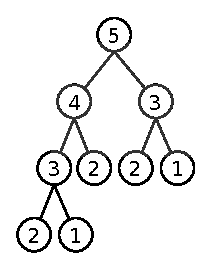
\includegraphics[width=0.2\textwidth]{images/fibonacciTree.eps}
  \end{center}
  \caption{Representación gráfica de las invocaciones generadas con $Fib(5)$.}
  \label{fig:Ch1fib}
\end{figure}

Ambas funciones realizan el cómputo del valor de Fibonacci para un número entero $N$. Sin embargo, la versión recursiva crea muchos ambientes recursivos durante la invocación de las funciones. Si se coloca de forma gráfica las invocaciones generadas con $Fib(5)$ de arriba hacia abajo, con enlaces que indiquen nuevos ambientes de programas, el resultado sería similar a como se observa en la Fig. \ref{fig:Ch1fib}. 

Se puede observar que existen invocaciones duplicadas (e.g. $Fib(2)$ se debe calcular 3 veces) que hacen ineficiente dicha implementación con respecto a una versión iterativa. Entonces, es importante evaluar el costo de construir algoritmos eficientes vs. legibilidad y simplicidad del código generado.

Es importante destacar que cualquier función recursiva se puede transformar en una función iterativa. Una forma de realizar esto es simulando la recursión con un Stack (ver la sección \ref{sec:recstack}, parte V para mayor detalle).

%%%%%%%%%%%%%%%%%%%%%%%%%%%%%%%%%%%%%%%%%%%%%%%%%%%%%%%%
\section{Ejercicios}

De forma natural, los algoritmos recursivos intentan solucionar un problema aplicando el concepto de divide y conquista. A continuación, una serie de ejercicios asociados al tema.

%%%%%%%%%%%%%%%%%%%%%%%%%%
\subsection{Imprimir una secuencia de números}

Se quiere imprimir una secuencia de números. Dado un número entero $n$ se desea que se imprima la serie de números de forma decreciente. Por ejemplo, para $n=9$ se quiere la secuencia:

9 8 7 6 5 4 3 2 1 0

La forma natural, es empleando un ciclo desde el valor $n$ hasta $0$ con decrementos de $1$ hasta que sea $0$. Empleando recursión la idea es construir un procedimiento que imprima el número $n$ que recibe como parámetro e invocar recursivamente al siguiente número de la secuencia con decrementos de $1$. El algoritmo se puede escribir de la siguiente forma:

\begin{lstlisting}[upquote=true, language=pseudo]
void MyPrint(Integer iN)
  if iN >= 0 then
    Print (iN)
    MyPrint (iN - 1)
  end
end
\end{lstlisting}

Se puede observar que la invocación inicial del procedimiento debe ser $MyPrint(9)$, e irá imprimiendo el valor y luego invocando a la función con $iN-1$ para realizar el decremento correspondiente. La finalización se determina por la condición $iN \ge 0$.

Supongamos realizar la misma tarea pero esta vez con la secuencia de forma inversa empleando recursión. Por ejemplo para $n=9$ se desea la secuencia:

0 1 2 3 4 5 6 7 8 9

Analizando un poco la solución de $MyPrint$, es posible intercambiar el orden de las instrucciones dentro del condicional tal que una vez invocado el último procedimiento, la siguiente instrucción sea imprimir el número. Esta operación se realiza de forma correcta gracias a que la recursión en sí misma crea los ambientes de ejecución donde el parámetro contiene el valor de $iN-1$ invocado por el ambiente anterior. Así, la función queda como:

\begin{lstlisting}[upquote=true, language=pseudo]
void MyPrint(Integer iN)
  if iNn >= 0 then
    MyPrint (iN - 1)
    Print (iN)
  end
end
\end{lstlisting}

Nótese que cuando el parámetro sea $iN=0$, se creará un nuevo ambiente recursivo donde el nuevo parámetro es $iN=-1$. En dicho ambiente, la condición será $false$ y no se ejecutará instrucción alguna, volviendo a la siguiente instrucción del punto de invocación cuando $iN=0$. La siguiente instrucción es $Print(iN)$ y así la secuencia se mostrará desde $0$ a $9$.

%%%%%%%%%%%%%%%%%%%%%%%%%%
\subsubsection{Potenciación}
La operación de potencia consiste en elevar el número $x$ a $y$ (i.e. $x^y$). Llamando a la función potencia $Pow$ que recibe dos parámetros que corresponden a la base y el exponente, se tiene que:

Pow (2, 4) = 16 \\
Pow (3, 4) = 81

Pensando en una versión iterativa de $Pow$, podemos escribirla como:

\begin{lstlisting}[upquote=true, language=pseudo]
function Pow (Integer iBase, iExp) : Integer
  if iExp == 0 then
    return 1
  end
  Integer iResult = iBase
  for Integer iI = 2 to iExp do
    iResult = iResult * iBase
  end
  return iResult
end
\end{lstlisting}

Para la versión recursiva se debe definir, los parámetros, el caso base y el caso recursivo. Queda claro que los parámetros solo son la base y el exponente:

\begin{lstlisting}[upquote=true, language=pseudo]
function Pow (Integer iBase, iExp) : Integer
\end{lstlisting}

Luego, se debe definir el caso base donde se conoce que $x^0 = 1$ y $x^1 = x$. Entonces se puede escribir como:

\begin{lstlisting}[upquote=true, language=pseudo]
function Pow (Integer iBase, iExp) : Integer
  if iExp == 0 then
    return 1
  elseif iExp == 1 then
    return iBase
\end{lstlisting}

Ahora para explorar el caso recursivo podemos analizar un poco la secuencia de operaciones que se emplean en el cálculo de la potencia:
Pow(2,0) = 1 \\
Pow(2,1) = 2 \\
Pow(2,2) = 2 * Pow(2,1) = 2 * 2 = 4 \\
Pow(2,3) = 2 * Pow(2,2) = 2 * 4 = 8 \\
Pow(2,4) = 2 * Pow(2,3) 2 * 8 = 16 \\
... \\
Pow(base, exp) = base * power(base, exp-1)

De esta forma, resulta sencillo traducir la fórmula al código para obtener la función Pow:

\begin{lstlisting}[upquote=true, language=pseudo]
function Pow (Integer iBase, iExp) : Integer
  if iExp == 0 then
    return 1
  elseif iExp == 1 then
    return iBase
  else
    return iBase * Pow(iBase, iExp-1)
  end
end
\end{lstlisting}

%%%%%%%%%%%%%%%%%%%%%%%%%%
\subsubsection{Convertir un decimal a binario}

Para hacer la conversión de un número de base 10 (decimal) a un número de base 2 (binario), se debe ir dividiendo el número decimal entre 2 y anotar en una columna a la derecha el resto (un 0 si el resultado de la división es par y un 1 si es impar). La lista de ceros y unos leídos de abajo a arriba es el resultado. En la Fig. \ref{fig:Ch1decbin} se muestra un ejemplo aplicado al decimal 19.

\begin{figure}[htpb!]
  \begin{center}
    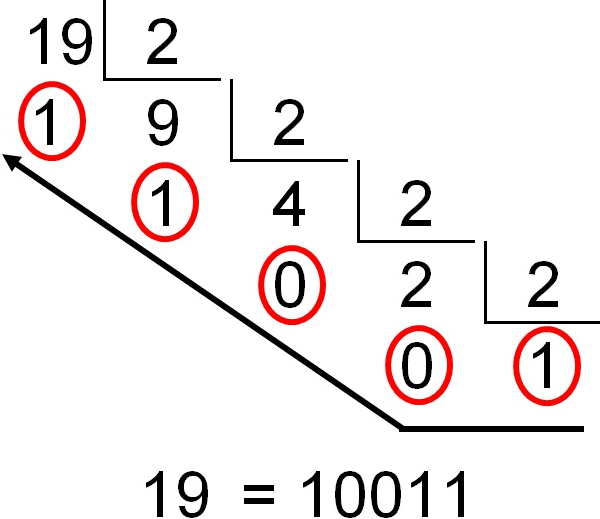
\includegraphics[width=0.2\textwidth]{images/decbin.png}
  \end{center}
  \caption{Proceso de conversión del número decimal 19 a su representación en binario.}
  \label{fig:Ch1decbin}
\end{figure}

Para construir la función recursiva se debe pensar en los 3 elementos primordiales de la recursión:
\begin{enumerate}
\item Caso Base: Cuando no se pueda dividir más el número entre 2
\item Caso Recursivo: Dividir el número siempre entre 2 (\textit{divide and conquer}) y emplear valor de su módulo para formar el número binario
\item Parámetros: Solo requiere el número decimal
\end{enumerate}

De esta forma, podemos escribir el siguiente procedimiento:

\begin{lstlisting}[upquote=true, language=pseudo]
void ToBinary (Integer iN)
  if iN < 2 then
    Print(iN)
  else
    ToBinary (iN div 2)
  end
  Print(iN mod 2)
end
\end{lstlisting}

Es importante destacar que es posible modificar el procedimiento tal que permita la conversión de base $10$ a base $k$ de forma muy simple.

%%%%%%%%%%%%%%%%%%%%%%%%%%%%%%%%%%%%%%%%%%%%%%%%%%%%%%%%
\section{Algoritmos}

En la literatura existe un conjunto de algoritmos muy empleados para entender la recursión como los algoritmos de ordenamiento QuickSort y MergeSort. Esta sección pretende complementar dichos algoritmos clásicos con algunos otros muy conocidos también:

\subsection{Collatz}
La conjetura de Collatz propuesta en 1937 (también conocido como el problema de $3n + 1$) define que dado un número natural $n$ si es par, se divide entre 2 para obtener $\frac{n}{2}$, si es impar se multiplica por 3 y se suma 1, $3 \times n + 1$. Este proceso se repite indefinidamente (siempre llegará a 1).
\begin{lstlisting}[upquote=true, language=pseudo]
void Collatz (Integer iN)
  Print (iN)
  if iN > 1 then
    if iN mod 2 == 0 then 
      Collatz (iN div 2) 
    else 
      Collatz (3*iN + 1)
    end
  end
end
\end{lstlisting}


\subsection{Búsqueda Binaria}

La búsqueda binaria busca un valor en una secuencia de elementos ordenados. La búsqueda binaria reduce un problema de tamaño $n$ a tamaño $\frac{n}{2}$ en cada iteración.

\begin{lstlisting}[upquote=true, language=pseudo]
function BinarySearchR (ref Array aValues of Integer[], Integer iNumber, iFirst, iLast) : Integer
  if iFirst > iLast then
    return -1
  end
  Integer iMiddle = (iFirst + iLast) div 2
  if aValues[iMiddle] == iNumber then
    return iMiddle
  end
  if aValues[iMiddle] < iNumber then
    BinarySearchR (ref aValues, iNumber, iMiddle + 1, iLast)
  end
  return BinarySearchR (ref aValues, iNumber, iFirst, iMiddle - 1)
end
\end{lstlisting}

\subsection{Hanoi}
	Las Torres de Hanoi es un juego inventado en 1883 que consiste en ocho discos de radio creciente que se apilan insertándose en una de las tres estacas de un tablero (ver Fig. \ref{fig:Ch1hanoi}). El objetivo del juego es crear la pila en otra de las estacas siguiendo tres reglas:
\begin{enumerate}
\item Solo se puede mover un disco a la vez
\item No puede haber un disco de mayor tamaño sobre uno de menor tamaño
\item Solo se puede mover un disco que este en el tope de una estaca
\end{enumerate}

\begin{figure}[htpb!]
  \begin{center}
    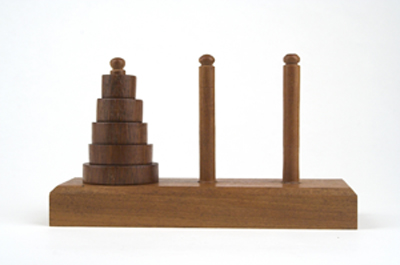
\includegraphics[width=0.5\textwidth]{images/hanoi.jpg}
  \end{center}
  \caption{Las Torres de Hanoi empleando 5 discos.}
  \label{fig:Ch1hanoi}
\end{figure}

\begin{lstlisting}[upquote=true, language=pseudo]
void Hanoi(Integer iN, iSource, iTarget, iTemp)
   if (iN <= 1) then
      MoveDisk(iSource, iTarget)	//just print "move from iSource to iTarget"
   else
      Hanoi (iN - 1, iSource, iTemp, iTarget)
      MoveDisk(iSource, iTarget)
      Hanoi (iN - 1, iTemp, iTarget, iSource)
   end
end
\end{lstlisting}

Cuenta la leyenda que en el antiguo templo de Brahma en Benarés se encontraba una cúpula que señalaba el centro del mundo. Bajo la cúpula se encontraba una bandeja sobre la cual existían tres agujas de diamante. Allí colocó Brahma 64 discos de oro en una de las agujas, siendo ordenados por tamaño: el mayor en la base y el menor arriba. Incansablemente, día tras día, los sacerdotes del templo mueven los discos haciéndoles pasar de una aguja a otra, de acuerdo con las leyes fijas e inmutables que dictó Brahma (las 3 reglas). El día en que los 64 discos hayan sido trasladados desde la aguja en que Brahma los puso a una cualquiera de las otras dos agujas, ese día la torre, el templo y el mundo entero desaparecerán. Para ello se requiere $2^{64}$ – 1 movimientos, y asumiendo que se emplea un segundo por cada movimiento, se necesitan 585 billones de años (127 veces la edad actual del sol).

\subsection{Palíndrome}

Un palíndrome es una palabra, una frase, un número o una secuencia de caracteres que se leída de izquierda a derecha o de derecha a izquierda, sean iguales. Por ejemplo las palabras reconocer, ananá, oro, arepera, entre otras son palabras palíndromes. Para el algoritmo determinaremos si una palabra es palíndrome.

\begin{lstlisting}[upquote=true, language=pseudo]
function IsPalindrome (String sWord, Integer iN) : Boolean
  if iN <= 1 then 
    return true
  elseif sWord[1] != sWord[iN] then
    return false
  else
    return IsPalindrome(sWord[2iN-1], iN-2)
  end
end
if IsPalindrome("Never Odd or Even") then
  Print ("Es Palíndrome")
 else
  Print ("No es Palíndrome")
end
\end{lstlisting}

\subsection{Invertir un número}

Esta función invierte el valor de un número entero y lo retorna. Emplea dos parámetros donde el primero corresponde al número a invertir y el segundo se emplea durante la recursión para mantener el cáĺculo parcial del número invertido.

\begin{lstlisting}[upquote=true, language=pseudo]
function Integer Reverse(Integer iN, iS)
 if iN == 0 then
   return iS
 else
  return Reverse(n div 10, s * 10 + n mod 10)
end
Print (Reverse(5831, 0)) //la salida es 1385
\end{lstlisting}

%%%%%%%%%%%%%%%%%%%%%%%%%%%%%%%%%%%%%%%%%%%%%%%%%%%%%%%%
\section{Ideas Finales}

\begin{itemize}
\item La recursión ofrece un mecanismo de solucionar problemas aplicando el principio de divide y conquista
\item Siempre se edbe garantizar la culminación del algoritmo (no olvidar la convergencia al caso base)
\item La recursión puede crear sub-problemas no tan pequeños, así como un número de invocaciones excesivas pudiendo ocasionar un desborde de pila
\item Cualquier función recursiva puede ser sustituida por una equivalente iterativa
\end{itemize}

%%%%%%%%%%%%%%%%%%%%%%%%%%%%%%%%%%%%%%%%%%%%%%%%%%%%%%%%
\section{Problemas}

\begin{enumerate}
\item Construya un algoritmo recursivo que permita hacer la división de dos números empleando restas sucesivas
\item Si existen 2 funciones recursivas que resuelven el problema A, ¿bajo cuáles criterios se selecciona la mejor solución?
\item Un número cumple con la propiedad de Goldbach si se puede escribirse como la suma de dos números primos. Defina una función que determine si un número natural cumple con esta propiedad
\item ¿Qué hace la siguiente función?
	\begin{lstlisting}[upquote=true, language=pseudo]
	function McCarthy (Integer iN)
    	if (iN > 100) then return iN - 10 end
    	else return McCarthy(McCarthy(iN + 11)) end
    end
	\end{lstlisting}
\item Haga una traza y determine que hace la función $Mistery$
\begin{lstlisting}[upquote=true, language=pseudo]
Integer Mystery (Integer a, int b)	//try using a = 3 and b = 4
  if b == 1 then
	return a
  else
    return a + Mystery (a, b - 1)
  end
end
\end{lstlisting}
\item Elabore un algoritmo recursivo que determine si existe una suma sucesiva de números igual a $k$, por ejemplo para el arreglo:
\begin{lstlisting}[upquote=true, language=pseudo]
Array aArr of Integer [] = {1,2,3,4,5,6}
\end{lstlisting}
\noindent se desea conocer si existe una suma sucesiva para 9. En este caso existe ya que 4+5=9, si se desea la suma de 7, esta es 3+4=7, para la suma de 10, 1+2+3+4=10. Ahora, para la suma de 8 es imposible puesto que el 2 y el 6 no son sucesivos
\end{enumerate}